\documentclass[10pt,twocolumn]{article}

\usepackage[letterpaper,top=0.34in,bottom=0.36in,left=0.36in,right=0.36in]{geometry}
\usepackage[T1]{fontenc}
\usepackage[utf8]{inputenc}
\usepackage{lmodern}
\usepackage{microtype}
\usepackage{titlesec}
\usepackage{titling}
\usepackage{amsmath}
\usepackage{amssymb}
\usepackage{booktabs}
\usepackage{graphicx}
\usepackage[hidelinks]{hyperref}
\usepackage[
  backend=biber,
  style=numeric,
  sorting=nyt,
  maxbibnames=4,
  giveninits=true
]{biblatex}

\addbibresource{references2.bib}
\graphicspath{{Figures/}}

\setlength{\parindent}{0pt}
\setlength{\parskip}{0.18em}
\setlength{\columnsep}{0.20in}
\setlength{\droptitle}{-4.8em}
\pretitle{\begin{center}\Large\bfseries}
\posttitle{\par\end{center}\vspace{-1.0em}}
\preauthor{\begin{center}}
\postauthor{\par\end{center}\vspace{-1.35em}}
\predate{}
\postdate{}
\titleformat{\section}{\bfseries\large}{\thesection}{0.55em}{}
\titlespacing*{\section}{0pt}{0.48em}{0.08em}
\setlength{\abovedisplayskip}{0.28em}
\setlength{\belowdisplayskip}{0.28em}
\setlength{\abovedisplayshortskip}{0.18em}
\setlength{\belowdisplayshortskip}{0.18em}

\AtEveryBibitem{%
  \ifboolexpr{not test {\iffieldundef{doi}} or not test {\iffieldundef{journaltitle}}}{%
    \clearfield{url}%
    \clearfield{eprint}%
    \clearfield{eprinttype}%
  }{}%
}
\AtBeginBibliography{\scriptsize}

\newcommand{\Runcited}{R_{\mathrm{uncited}}}

\title{Grounding quality measurement for orchestrated AI reasoning chains:
       evidence-binding rate as an evaluation primitive for world model systems}
\author{Gil Raitses \\ \small aimez.ai}
\date{}

\begin{document}

\maketitle

\fontsize{8.45}{9.25}\selectfont

\begin{abstract}
AI systems that reason about physical or scientific domains routinely produce outputs
containing scientific claims without citing their generating evidence. $\Runcited$ --- the
fraction of scientific sentences in a system's output that carry no bound citation --- is a
formal evaluation primitive for AI reasoning quality. Using a reproducible 8-scenario parallel
benchmark against the Gemini Interactions API with Google Maps grounding on marine science
queries, Maps-only geospatial grounding achieves 60--100\% uncited across query types.
Injecting a structured orchestrated skill-dispatch step-log as RAG context reduces $\Runcited$
to 0\%, demonstrating that planning traces eliminate uncited claims by converting open-domain
science queries into closed artifact-reference queries. The RAG lift hierarchy (step-log $>$
structured data $>$ narrow context $>$ unstructured) functions as a diagnostic for grounding
architecture quality: context that binds the query to a complete reasoning trace eliminates
uncited claims; narrowly structured context does not. The extension of this benchmark to AI
planning systems whose intermediate representations are required to be grounded in their
generating sensor observations is examined.
\end{abstract}

\section{The evidence-binding gap in AI reasoning systems}

AI systems that generate natural language outputs about scientific or physical domains make claims
that require empirical grounding. When a language model responds to a question about orca encounter
likelihood at Haro Strait, it may correctly name the relevant salmon corridor, acoustic monitoring
network, and behavioral studies --- but without binding any of these claims to their generating
observations, prior analyses, or data artifacts. The response is fluent and plausible; it is not
evidentially accountable.

This is the evidence-binding gap: the structural disconnection between a system's stated claims and
the observations, methods, and experiments that would make those claims verifiable. The gap is not a
matter of factual accuracy per se --- a claim may be broadly correct while still carrying no bound
evidence. It is a matter of verifiability: a judge, steward, or downstream system cannot determine
whether the claim was produced by accessing ground-truth data or by reproducing a plausible-sounding
pattern from training.

Prior work on RAG hallucination reduction~\cite{arxiv230915217,arxiv230514627,arxiv240115884,arxiv231109533}
establishes that retrieval-augmented generation reduces factual error rates and that citation generation
can be automated. However, this literature focuses on whether RAG improves accuracy, not on whether
the improvement comes from evidence binding --- from the system's outputs being traceable to their
generating context --- versus improved parametric knowledge activation.

The geospatial grounding baseline makes this distinction concrete. Google Maps grounding achieves high
citation density for place-of-interest queries. For marine science evidence queries --- the same domain,
but requiring scientific rather than place-level grounding --- Maps grounding resolves 0 of 25 citations
to scientific or dataset sources. NOAA fisheries data, the Center for Whale Research census, Chinook
salmon migration corridors, and acoustic hydrophone recordings are all generated as claims but remain
entirely uncited. The system knows about these phenomena from training; it cannot bind its claims to
verifiable data artifacts.

$\Runcited$ --- the fraction of scientific sentences in a system's output with no bound
citation --- is the measurement primitive that makes this gap quantitative, reproducible, and
architecture-diagnostic.

\section{$\Runcited$ as a formal evaluation metric}

\subsection{Definition}

Let $S$ be the set of sentences in a system's output. Define $S_\mathrm{sci} \subseteq S$ as the
sentences containing scientific or quantitative markers. For each sentence $s \in S_\mathrm{sci}$,
let $\mathrm{cited}(s)$ be the indicator that $s$ names at least one entity appearing in the bound
citation set $C$.

\begin{equation}
\label{eq:runcited}
\Runcited = \frac{|\{ s \in S_\mathrm{sci} : \neg\,\mathrm{cited}(s) \}|}{|S_\mathrm{sci}|}
\end{equation}

$\Runcited = 0$ when every scientific sentence names a bound citation. $\Runcited = 1$ when no
scientific sentence does. It is undefined when $|S_\mathrm{sci}| = 0$.

\subsection{Properties}

$\Runcited$ has four properties that make it useful as an evaluation primitive.

\textbf{Claim-level granularity.} The metric operates at the sentence level. A response with 10
scientific sentences and 9 bound citations still has $\Runcited = 0.1$, distinguishing it from
response-level pass/fail metrics.

\textbf{Architecture-diagnostic.} Two systems with the same surface accuracy can have very different
$\Runcited$ values depending on whether their reasoning traces are passed as context to the language
model. The metric discriminates between evidence-bound and parametric-knowledge-based claim generation.

\textbf{Reproducible.} $\Runcited$ is computed from the raw API output. No human annotation is
required. The scientific marker set is implemented as a regex over domain-specific technical terms.

\textbf{Model-independent.} $\Runcited$ can be applied to any language model's output. It measures
the binding between output and context, not internal model behavior.

\subsection{Relation to prior evaluation frameworks}

The Ragas framework~\cite{arxiv230915217} evaluates faithfulness (whether claims are supported by
retrieved context), answer relevancy, and context precision. These metrics require a reference context.
$\Runcited$ measures a weaker but more deployable condition: whether the model's output names sources
in the context it was given, without requiring a predefined reference set.

The ALCE benchmark~\cite{arxiv230514627} evaluates citation generation at the claim level. $\Runcited$
is complementary: it measures the rate of claims carrying no citation at all, regardless of citation
validity.

$\Runcited$ is also distinct from explainable-AI evaluation, which concerns the transparency of a
model's decision process rather than the binding of its output to gathered evidence~\cite{clinciu2019survey},
and from reasoning-chain evaluation, which scores the internal correctness and informativeness of
intermediate steps rather than their traceability to artifacts~\cite{arxiv230410703}.

\section{Benchmark methodology and results}

\subsection{Setup}

The benchmark uses the Gemini Interactions API (gemini-3.5-flash, Api-Revision: 2026-05-20) with
\texttt{google\_maps} tool at San Juan Islands coordinates (48.5465, $-$123.03). Eight scenarios run
in parallel via Python asyncio (\texttt{tools/testing/grounding\_parallel\_rag.py}), each submitting a
distinct query with a distinct RAG context type. Run date: 2026-06-24.

\subsection{Scenarios}

\begin{center}
\small
\begin{tabular}{@{}lll@{}}
\toprule
\# & Context injected & Query type \\
\midrule
1 & Maps-only (none) & Where are SRKWs seen + evidence \\
2 & Live gate data & Same + gate framing \\
3 & Cell provenance & Cell intensity + kernels \\
4 & Surface planner step-log & Gates blocking promotion \\
5 & Maps-only (none) & Sighting check \\
6 & Sighting-assist output & Same + orcast data \\
7 & Maps-only (none) & Shore whale watching plan \\
8 & Hotspot probability data & Same + orcast forecast \\
\bottomrule
\end{tabular}
\end{center}

\subsection{Results}

\begin{center}
\small
\begin{tabular}{@{}llr@{}}
\toprule
Scenario & Context & $\Runcited$ \\
\midrule
4 & Planner step-log & \textbf{0\%} \\
8 & Hotspot data & 75\% \\
1 & Maps-only orca & 60\% \\
7 & Maps-only trip & 100\% \\
2 & Gate context & 100\% \\
3, 5, 6 & Provenance / sighting & 100\% \\
\bottomrule
\end{tabular}
\end{center}

Scenario~4 achieves $\Runcited = 0\%$. Scenario~8's hotspot data lowers $\Runcited$ by 25~pp
relative to the same trip-planning query without it (Scenario~7, 100\%), partially substituting
for science claims.
\section{The RAG lift hierarchy as a grounding architecture diagnostic}

The 8-scenario results reveal a diagnostic structure:

\begin{center}
\small
\begin{tabular}{@{}ll@{}}
\toprule
Context type & $\Runcited$ \\
\midrule
Step-log (complete reasoning trace) & 0\% \\
Structured domain data (hotspots) & 75\% \\
Maps-only baseline & 60--100\% \\
Narrow structured data (gates) & 100\% \\
\bottomrule
\end{tabular}
\end{center}

This is not a function of data volume but of structural alignment between context type and the science
claims the model otherwise generates.

\textbf{Full grounding (step-log):} The planner step-log records skills dispatched, panels selected,
and artifacts referenced; the query is answerable from those references without open-domain science
claims. $\Runcited$ collapses to 0\% because $|S_\mathrm{sci}| = 0$.

\textbf{Partial grounding (hotspot data):} Structured probability data substitutes for some generic
science claims; the remaining 75\% uncited rate is ecology claims the hotspot data does not cover.

\textbf{No grounding (gate data):} Gate data covers statistical test outcomes only; the model still
generates broader ecology claims gate data does not address.

Context type is a grounding affordance that shapes which claims become evidence-bound~\cite{davis2023affordances};
complete reasoning traces eliminate uncited claims; narrow structured context does not. The diagnostic
ports to any domain where the reasoning trace can be injected as context; eRAG retrieval
evaluation~\cite{arxiv240413781} would show the same pattern --- only step-log documents are fully utilized.

The Citation-Enhanced Generation framework~\cite{arxiv240216063} demonstrates that post-hoc citation
binding reduces hallucination in chatbots. The hierarchy finding complements this: pre-hoc trace
injection eliminates the class of queries that citation binding must address.

\section{Extension to AI planning systems}

\subsection{The step-log as a planning trace}

The surface planner step-log that achieves $\Runcited = 0\%$ in Scenario~4 has the
structure of a planning trace. The agent received a query, resolved a configuration,
dispatched skills, and produced a plan. The step-log records every intermediate state:
which skills ran, what their outputs were, and what the final plan consists of. When
this trace is injected as RAG context, the language model answers from the trace's
artifact references rather than from world knowledge. $\Runcited = 0\%$ because the
trace transforms the query from open-domain science to closed artifact-reference.

The paper ``Reasoning with Language Model is Planning with World Model''~\cite{arxiv230514992}
explicitly frames LLM reasoning steps as world-state traces and proposes evaluating whether
those states are accurate. The evaluation problem $\Runcited$ addresses is the evidence-binding
dimension of this: not whether the intermediate states are accurate, but whether each state
is traceable to the observations that produced it. TRACE~\cite{arxiv240611460} demonstrates
that constructing knowledge-grounded reasoning chains from structured context eliminates
irrelevant retrieval noise in multi-hop queries; the orcast step-log is this structure applied
to skill-dispatch interactions. Chain-of-Thought evaluation~\cite{arxiv220111903} confirms
that intermediate reasoning steps are causally important for correct final outputs, supporting
the claim that step-log quality measurement is foundational to planning system evaluation.

\subsection{Applying $\Runcited$ to planning systems}

The benchmark methodology in Section~4 is directly portable to any AI planning system whose
interactions produce a structured trace. For a planning system that receives a query about a
physical or scientific domain, dispatches skills or sensors to gather current-state information,
produces a plan or action sequence based on gathered context, and narrates the plan with
references to gathered artifacts: inject the planning trace as RAG context to a language model,
ask a domain-specific question, and measure $\Runcited$ on the response. When the trace binds
the query to artifact references, $\Runcited$ approaches 0\%. When the trace is sparse or
unstructured, $\Runcited$ remains high.

The RAG lift hierarchy (Section~5) provides the diagnostic: step-log context achieves full
grounding; structured domain data achieves partial lift; narrow structured data achieves no
lift. This hierarchy is a property of context-type alignment with the science claims the
model would otherwise generate, not a property of context volume. The Ragas framework
~\cite{arxiv230915217} measures faithfulness separately from answer relevancy; $\Runcited$
measures a simpler, deployable condition that precedes both: whether claims are cited at all.

\section{Limits and falsification}

\subsection{Scope limits}

\textbf{Domain specificity.} The benchmark uses marine science queries. Extension to other domains
requires updating the science marker regex for that domain's technical vocabulary.

\textbf{Model dependence.} Results were produced with gemini-3.5-flash (2026-06-24). A model with
stronger domain-specific knowledge may generate fewer science claims.

\textbf{$\Runcited$ does not measure semantic accuracy.} A claim that is cited to a bound artifact
but semantically wrong is not captured. Extension to factual accuracy requires a reference
ground truth.

\textbf{Step-log quality dependence.} $\Runcited = 0\%$ requires a complete, structured step-log;
sparse or malformed traces would not achieve the same result.

\subsection{Falsification conditions}

\begin{center}
\small
\begin{tabular}{@{}p{4.5cm}p{3.8cm}@{}}
\toprule
Claim & Falsifying condition \\
\midrule
Step-log injection achieves $\Runcited = 0\%$ & Step-log-injected query produces uncovered science claims \\
Hierarchy is stable across query types & Different Scenario~4 query yields high $\Runcited$ \\
Gate context achieves no lift & Gate data injection covers generated science claims \\
$\Runcited$ diagnoses architecture quality & Two architecturally different systems produce identical hierarchies \\
\bottomrule
\end{tabular}
\end{center}

\subsection{Extension path}

Multi-domain validation: run the benchmark on pedestrian routing (pax), clinical care, and
manufacturing. World model evaluation: apply the benchmark to JEPA-based world models
(V-JEPA~\cite{arxiv240408471}) and measure whether planning trace injection reduces $\Runcited$.
Semantic accuracy addition: add a second metric for whether cited claims are factually accurate
relative to their bound artifacts.

\subsection{The benchmark gap in existing physical-world evaluation}

Physical-world AI benchmarks evaluate task completion or prediction accuracy without auditing
intermediate claim binding. PHYRE~\cite{arxiv190805656} measures physical reasoning via puzzle
solve rate. STAR~\cite{arxiv240509711} evaluates situated reasoning in real-world videos via
question answering accuracy. ThreeDWorld~\cite{arxiv210314025} measures embodied planning by
object transport success rate. TravelPlanner~\cite{arxiv240201622} evaluates language agent
planning by plan validity. The comprehensive Embodied AI survey~\cite{arxiv240706886} categorizes
evaluation as navigation, interaction, manipulation, and reasoning accuracy. None measures whether
intermediate reasoning claims are bound to their generating sensor observations. EWOK~\cite{arxiv240509605}
tests world modeling via plausibility matching. The need for evaluation primitives beyond functional
task success has a precedent: human-robot interaction required psychological benchmarks to capture
what task-completion metrics omit~\cite{kahn2007benchmarks}. $\Runcited$ provides the missing
primitive for evidence binding.

\subsection{World model evaluation as a future extension}

A natural extension is to apply this benchmark to world model planning systems whose design
explicitly requires sensor-grounded intermediate representations. LeCun's autonomous machine
intelligence architecture~\cite{arxiv230602572} specifies that the world model module must
learn to represent the information content of the percept that is relevant for predicting
future states --- a grounding requirement on intermediate representations. Joint-embedding
predictive architectures, from I-JEPA~\cite{arxiv230108243} to V-JEPA~\cite{arxiv240408471}, and
Image World Models~\cite{arxiv240300504} are evaluated on downstream accuracy on image and video
benchmarks; no claim-level evidence binding metric is proposed.
Whether $\Runcited$ on JEPA planning traces reproduces Section~5's diagnostic hierarchy is an open
empirical question. Section~4's methodology requires only a structured planning trace; running it on
world model outputs needs no architectural change.


\clearpage
\nocite{*}
\printbibliography[title={References}]

\appendix
\section*{Appendix: Figures}

\begin{figure}[h]
  \centering
  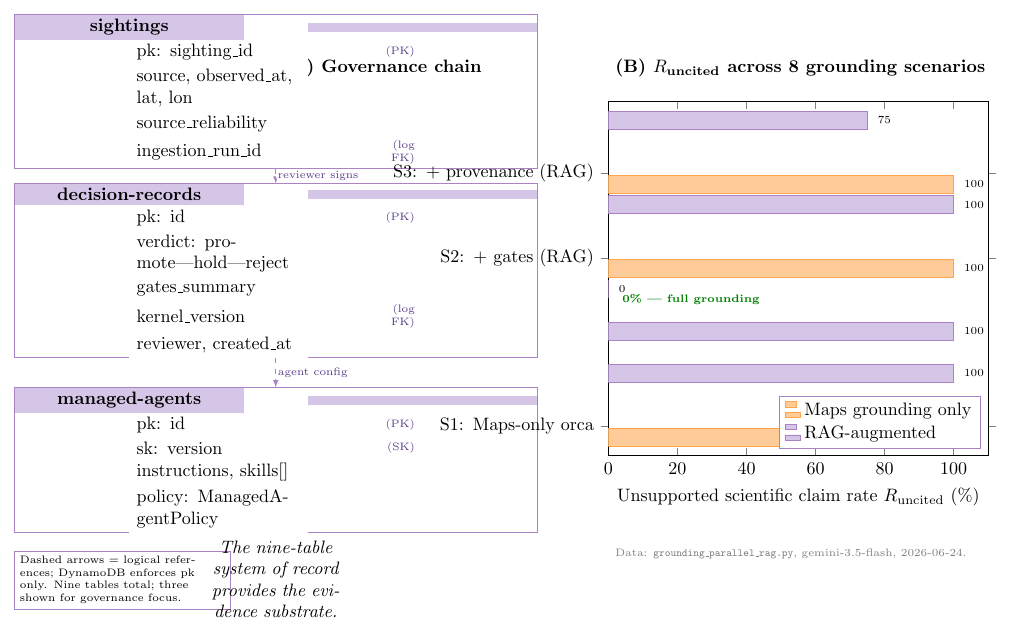
\includegraphics[width=\linewidth]{fig-mp1.png}
  \caption{\textbf{Evidence-binding failure and its measurement.}
    (A) The orcast governance chain: sightings, decision-records, and managed-agents
    in DynamoDB. (B) $\Runcited$ across eight grounding scenarios. Maps-only baseline:
    60--100\%. Surface planner step-log (Scenario~4): $\Runcited = 0\%$.
    Data: \texttt{grounding\_parallel\_rag.py}, gemini-3.5-flash, 2026-06-24.}
  \label{fig:problem}
\end{figure}

\begin{figure}[h]
  \centering
  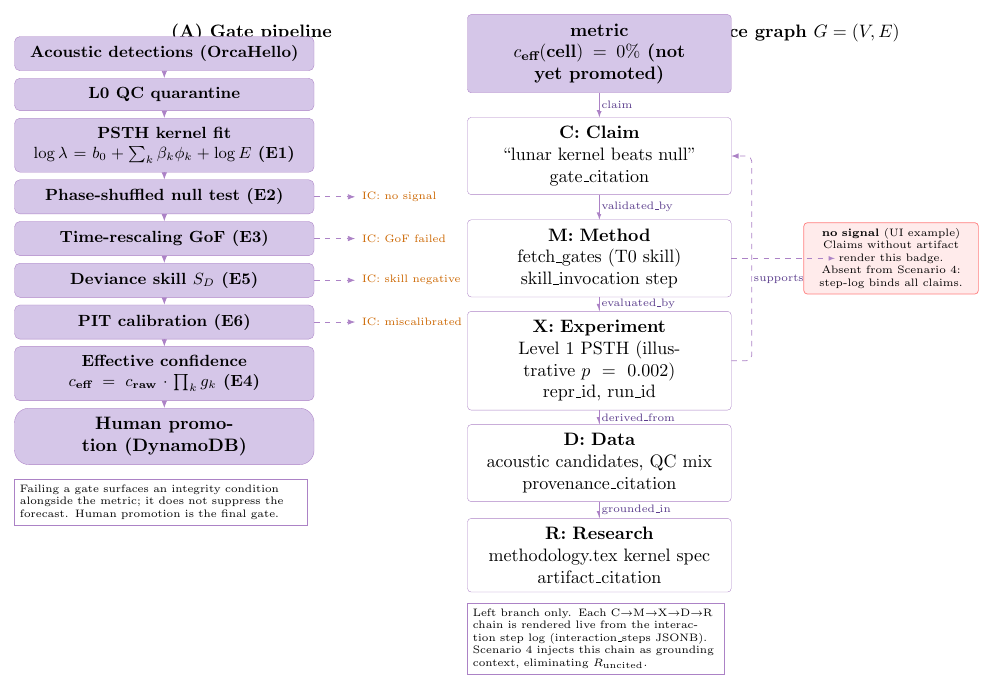
\includegraphics[width=\linewidth]{fig-mp2.png}
  \caption{\textbf{The mechanism that produces $\Runcited = 0\%$.}
    (A) Gate pipeline from acoustic detections to displayed confidence.
    (B) Provenance graph $G=(V,E)$: Claim (C) $\to$ Method (M) $\to$
    Experiment (X) $\to$ Data (D) $\to$ Research (R). Claims without
    a bound artifact render the ``no signal'' badge.
    Scenario~4 eliminates $\Runcited$ because the planner step-log binds
    every claim to an artifact reference.}
  \label{fig:mechanism}
\end{figure}

\begin{figure}[h]
  \centering
  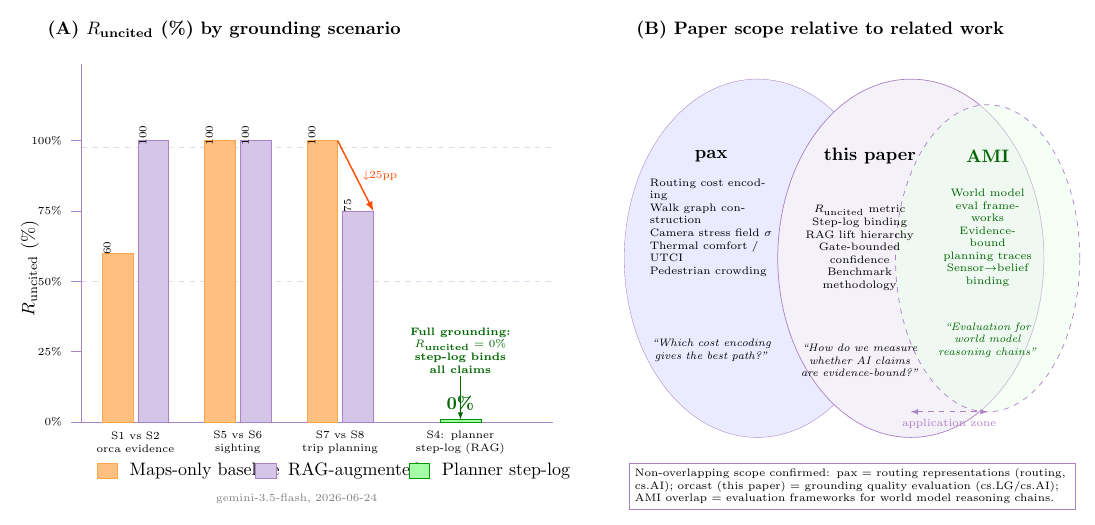
\includegraphics[width=\linewidth]{fig-mp3.png}
  \caption{\textbf{Grounding quality hierarchy and paper scope.}
    (A) $\Runcited$ for baseline vs RAG-augmented scenarios. The surface
    planner step-log (green, 0\%) dominates; hotspot data provides partial
    lift (S7$\to$S8); gate context provides no lift.
    (B) Paper scope: this paper addresses grounding evaluation methodology
    (center), distinct from pedestrian routing cost representations (pax, left),
    and directly applicable to world model evaluation infrastructure (AMI, right).}
  \label{fig:scope}
\end{figure}


\end{document}
